\documentclass[12pt]{article}
\usepackage[english]{babel}
\usepackage{amsmath,amsfonts,amsthm,amssymb,bm}
%\usepackage{longtable}
\usepackage{booktabs}
\usepackage{afterpage}
\usepackage{etoolbox}
\usepackage[applemac]{inputenc}
\usepackage{textcomp}
\usepackage[usenames,dvipsnames,svgnames,table]{xcolor}
\usepackage{todonotes}
\usepackage{menukeys}
\usepackage{afterpage}
\usepackage{pdflscape}
\usepackage{mathtools}
\usepackage{mathptmx}% http://ctan.org/pkg/mathptmx
\DeclareMathOperator{\E}{\mathbb{E}} %Declare expectations simply as \E
\usepackage{libertine} %For empty horizontal spaces
\usepackage[capposition=top]{floatrow} %This is used to use notes below figures. Command is float row. 
\usepackage{amsthm}
\def\changemargin#1#2{\list{}{\rightmargin#2\leftmargin#1}\item[]}
\let\endchangemargin=\endlist
\DeclareMathOperator{\var}{var}
\DeclareMathOperator{\cov}{cov}






%Style of font:
\usepackage{tgpagella}

%Defining the necessary symbol for independence:
\newcommand\independent{\protect\mathpalette{\protect\independenT}{\perp}}
\def\independenT#1#2{\mathrel{\rlap{$#1#2$}\mkern2mu{#1#2}}}

\usepackage{hyperref}
\hypersetup{
  letterpaper,
  bookmarksnumbered,
  bookmarksopen,
  bookmarksopenlevel=0,
  colorlinks,
% for colors, check package xcolor
%   anchorcolor=anchorcolor,
    citecolor=blue,
%   linkcolor=linkcolor,
	pdfauthor={Rodrigo Azuero Melo},
	pdftitle={Evaluating Early Childhood Interventions},
	pdfsubject={},
	pdfkeywords={},
%   plainpages=false,
%   urlcolor=urlcolor
}
\usepackage{comment}
\usepackage{apacite}
\usepackage{graphicx}
\usepackage{rotating}
\usepackage{lscape}
\usepackage{multirow}
\usepackage{hvfloat}
\usepackage{threeparttable}
\usepackage{bbm}
\usepackage{caption}
\usepackage{float}

\usepackage{chngcntr} %Change number figures in the appendix
%\usepackage{keyval}
\usepackage{enumerate}
%\usepackage{floatrow}
%\usepackage[captionskip=-2pt]{subfig}
%\usepackage{subfig}
\usepackage[letterpaper,centering]{geometry}
\usepackage{setspace}
\usepackage{amsmath}
\usepackage{caption}
\usepackage{multicol} %Allows to use multiple columns through the document


\usepackage{python}%Use python

\long\def\/*#1*/{}  %%This is for defining the function comment in multiple lines with \/* starting and */ finishing. 
\onehalfspacing

%\usepackage[thmmarks, thref, hyperref]{ntheorem}
%%\usepackage[thmmarks, thref, hyperref]{ntheorem}
%
%\theoremsymbol{\ensuremath{_\Box}}
\newtheorem{definition}{Definition}
\newtheorem{example}{Example}
\newtheorem{theorem}{Theorem}
\newtheorem{lemma}{Lemma}
\newtheorem{proposition}{Proposition}
\newtheorem{corollary}{Corollary}
\newtheorem{problem}{Problem}
\newtheorem{axiom}{Axiom}
\newtheorem{remark}{Remark}[section]
%
%\theoremsymbol{\ensuremath{_\blacksquare}}
%\theorembodyfont{\normalfont}
%\newtheorem*{proof}{Proof}
%\newtheorem*{claim}{Claim}

%\linespread{value}-->This is good to increase the spread between lines. 

\usepackage[usenames,dvipsnames]{xcolor}
\usepackage{ifthen}
\usepackage{listings}
\usepackage{courier}

\definecolor{light-gray}{gray}{0.90}
\definecolor{MyDarkGreen}{rgb}{0.0,0.4,0.0}

% For faster processing, load Matlab syntax for listings
\lstloadlanguages{Matlab}%
\lstset{language=Matlab,
        frame=single,
        basicstyle=\small\ttfamily,
        keywordstyle=[1]\color{Blue}\bf,
        keywordstyle=[2]\color{Purple},
        keywordstyle=[3]\color{Blue}\underbar,
        identifierstyle=,
        commentstyle=\usefont{T1}{pcr}{m}{sl}\color{MyDarkGreen}\small,
        stringstyle=\color{Purple},
        showstringspaces=false,
        tabsize=5,
        % Put standard MATLAB functions not included in the default
        % language here
        morekeywords={xlim,ylim,var,alpha,factorial,poissrnd,normpdf,normcdf},
        % Put MATLAB function parameters here
        morekeywords=[2]{on, off, interp},
        % Put user defined functions here
        morekeywords=[3]{FindESS},
        morecomment=[l][\color{Blue}]{...},
        numbers=left,
        firstnumber=1,
        numberstyle=\tiny\color{Blue},
        stepnumber=5
        }



\newcommand{\indexfonction}[1]{\index{#1@\texttt{#1}}}

\usepackage{subfig}

\renewcommand{\thesubfigure}{\thefigure.\arabic{subfigure}}
\captionsetup[subfigure]{labelformat=simple,labelsep=colon,
listofformat=subsimple}
\captionsetup{lofdepth=2}
\makeatletter
\renewcommand{\p@subfigure}{}
\makeatother
\setlength\parindent{10pt}

\renewcommand{\thesubtable}{\thetable.\arabic{subtable}}
\captionsetup[subtable]{labelformat=simple,labelsep=colon,
listofformat=subsimple}
\makeatletter
\renewcommand{\p@subtable}{}
\makeatother
\captionsetup[subfigure]{position=bottom}


%\def\sf@ifpositiontop{%
%\ifx\caption@position\@firstoftwo \let\next\@firstoftwo \else
%\let\next\@secondoftwo \fi \next}
%Margin modify margenes modificar
\newgeometry{left=3.0cm,bottom=2.0cm, right=3.0cm, top=3cm}
%\graphicspath{{Figures/}}
\title{\vspace{-3cm}Figures}
\author{Rodrigo Azuero}
\date{\today}

\begin{document}
\maketitle




%-----------------%
%Body of text %
%----------------%

\doublespacing
%Main body of the article
AfterTaxProfitPercentile


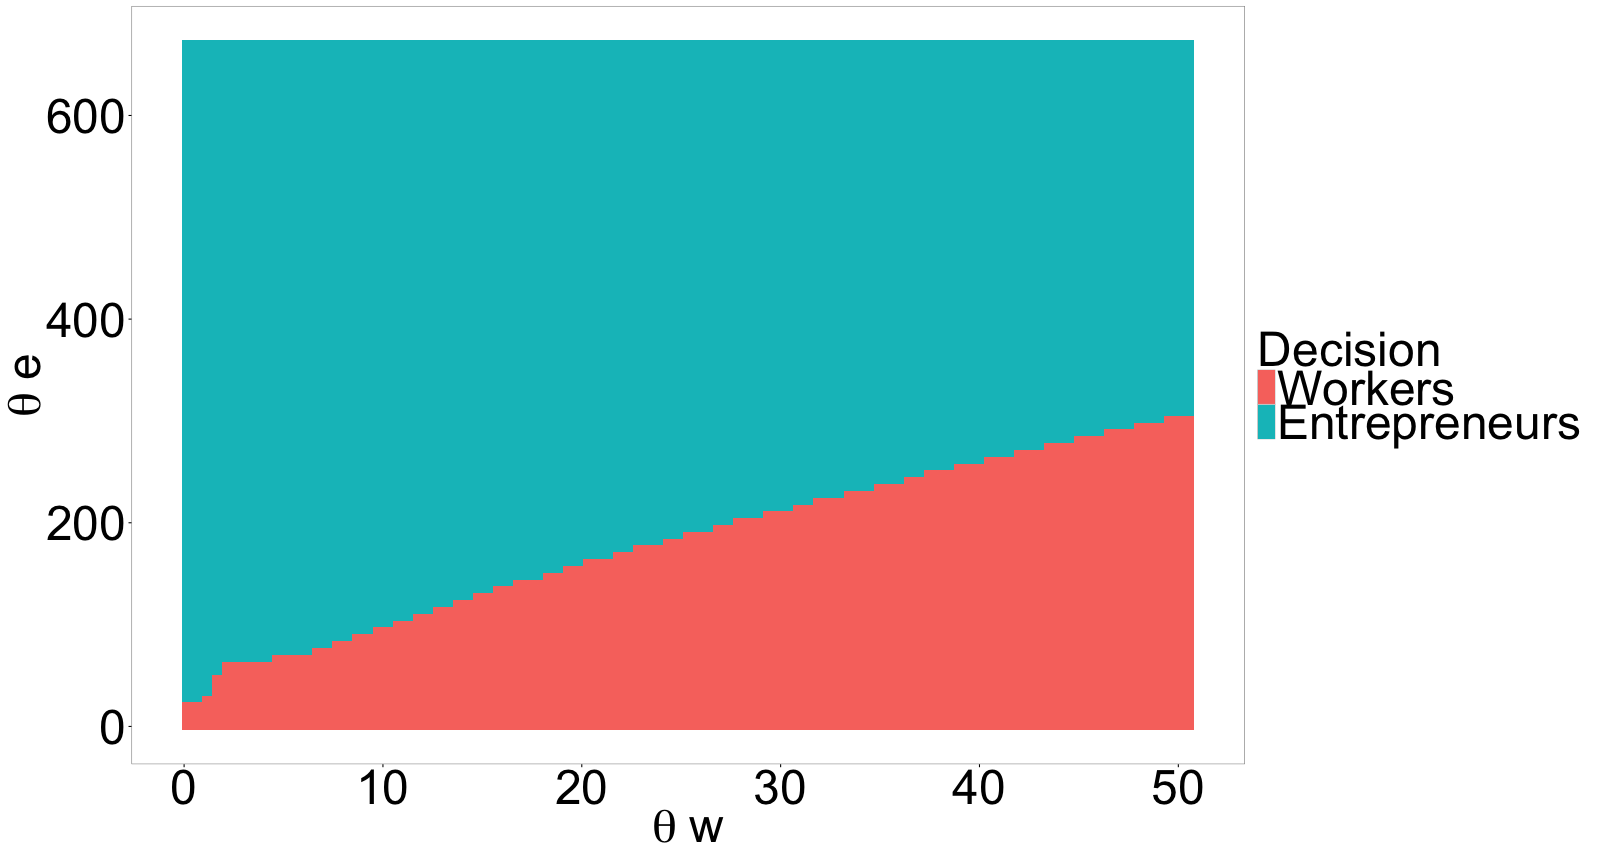
\includegraphics[width=1\textwidth]{/Users/rodrigoazuero/Dropbox/OptmalTaxationShared/Data/git/OptimalTaxation/TheoreticalMoments/EntreprenDecision.png}


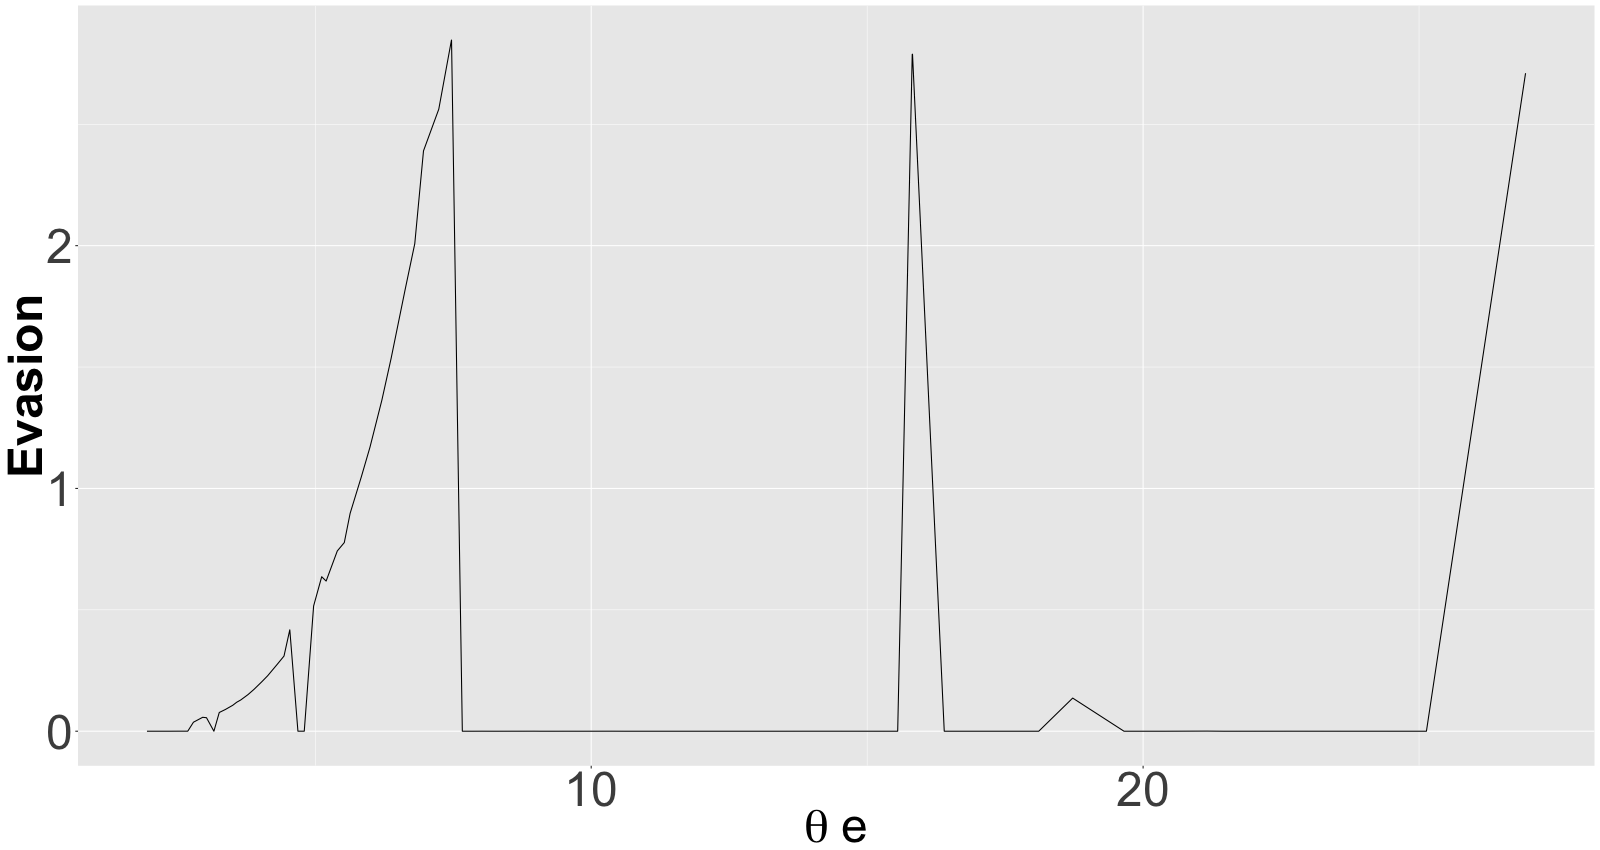
\includegraphics[width=1\textwidth]{/Users/rodrigoazuero/Dropbox/OptmalTaxationShared/Data/git/OptimalTaxation/TheoreticalMoments/EvasionProportion.png}

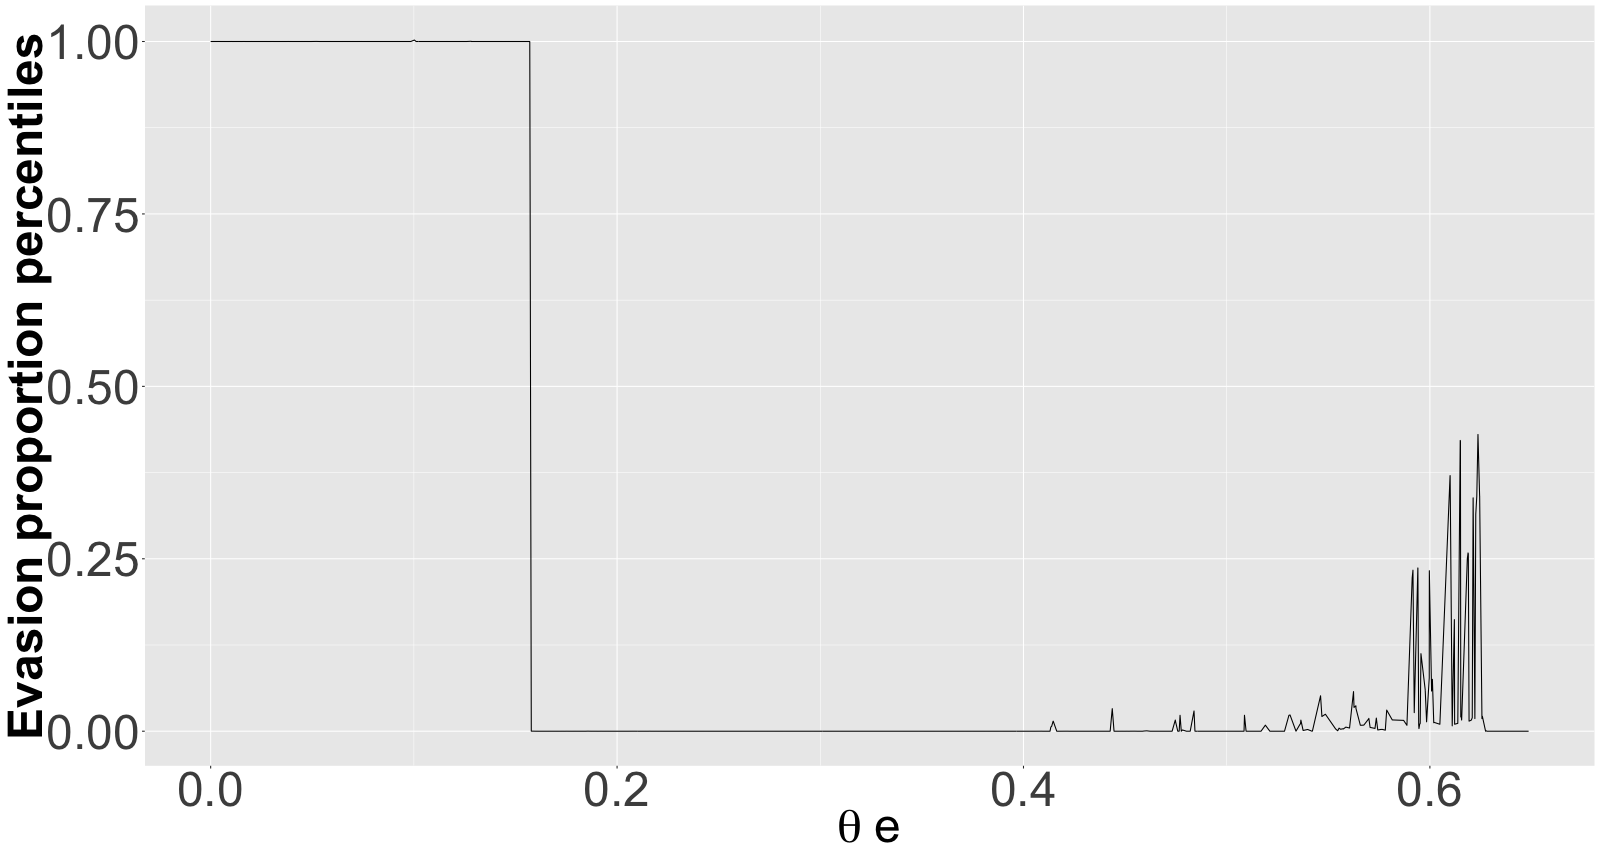
\includegraphics[width=1\textwidth]{/Users/rodrigoazuero/Dropbox/OptmalTaxationShared/Data/git/OptimalTaxation/TheoreticalMoments/EvasionProportionPercentiles.png}

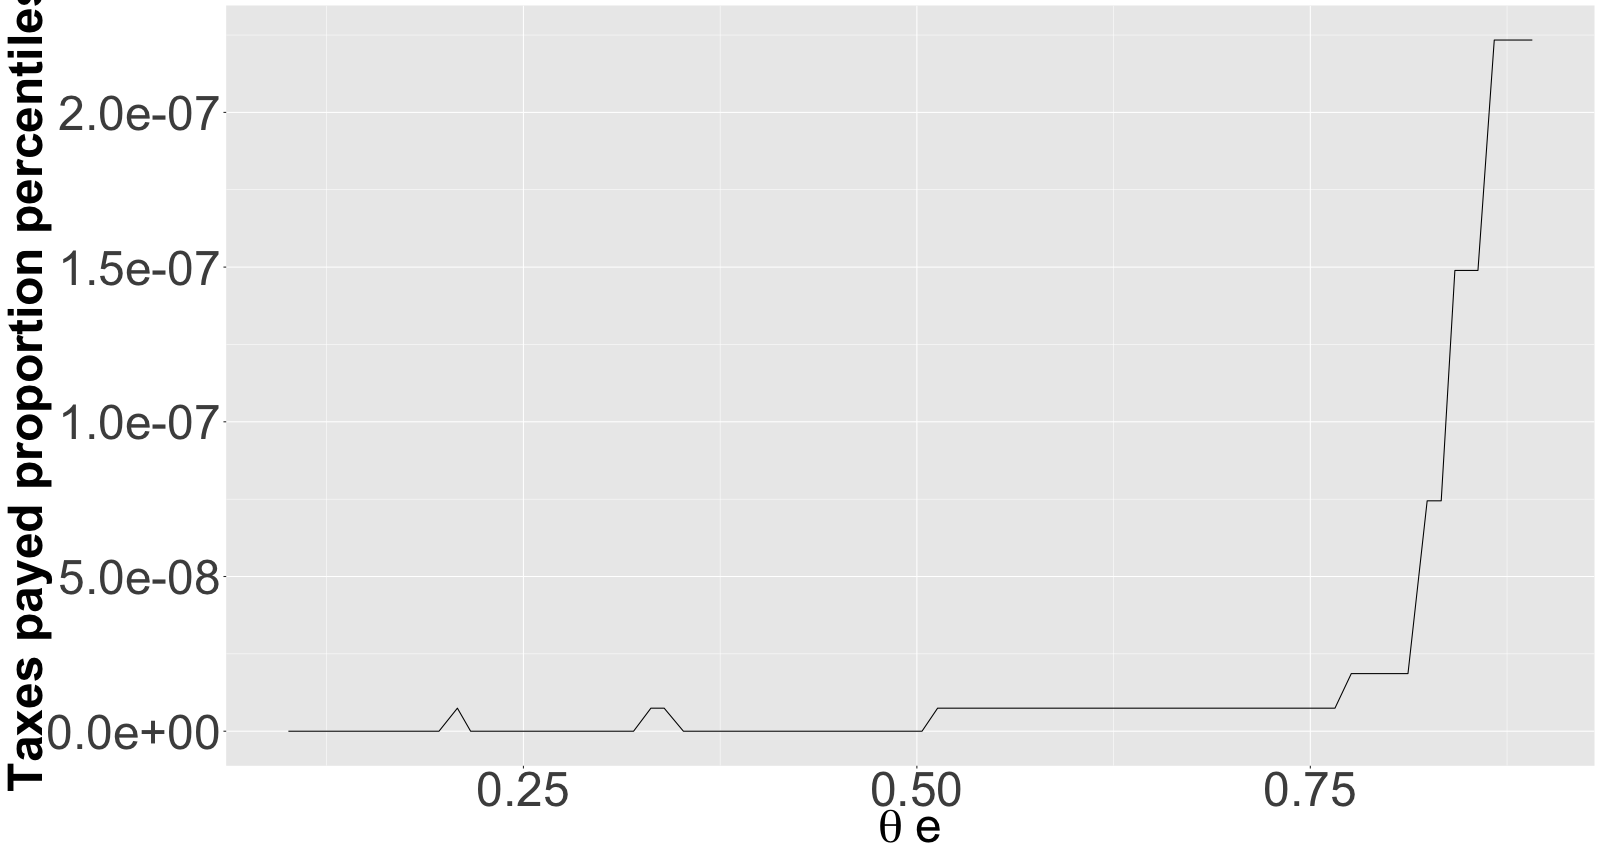
\includegraphics[width=1\textwidth]{/Users/rodrigoazuero/Dropbox/OptmalTaxationShared/Data/git/OptimalTaxation/TheoreticalMoments/TaxesPayedProportion.png}

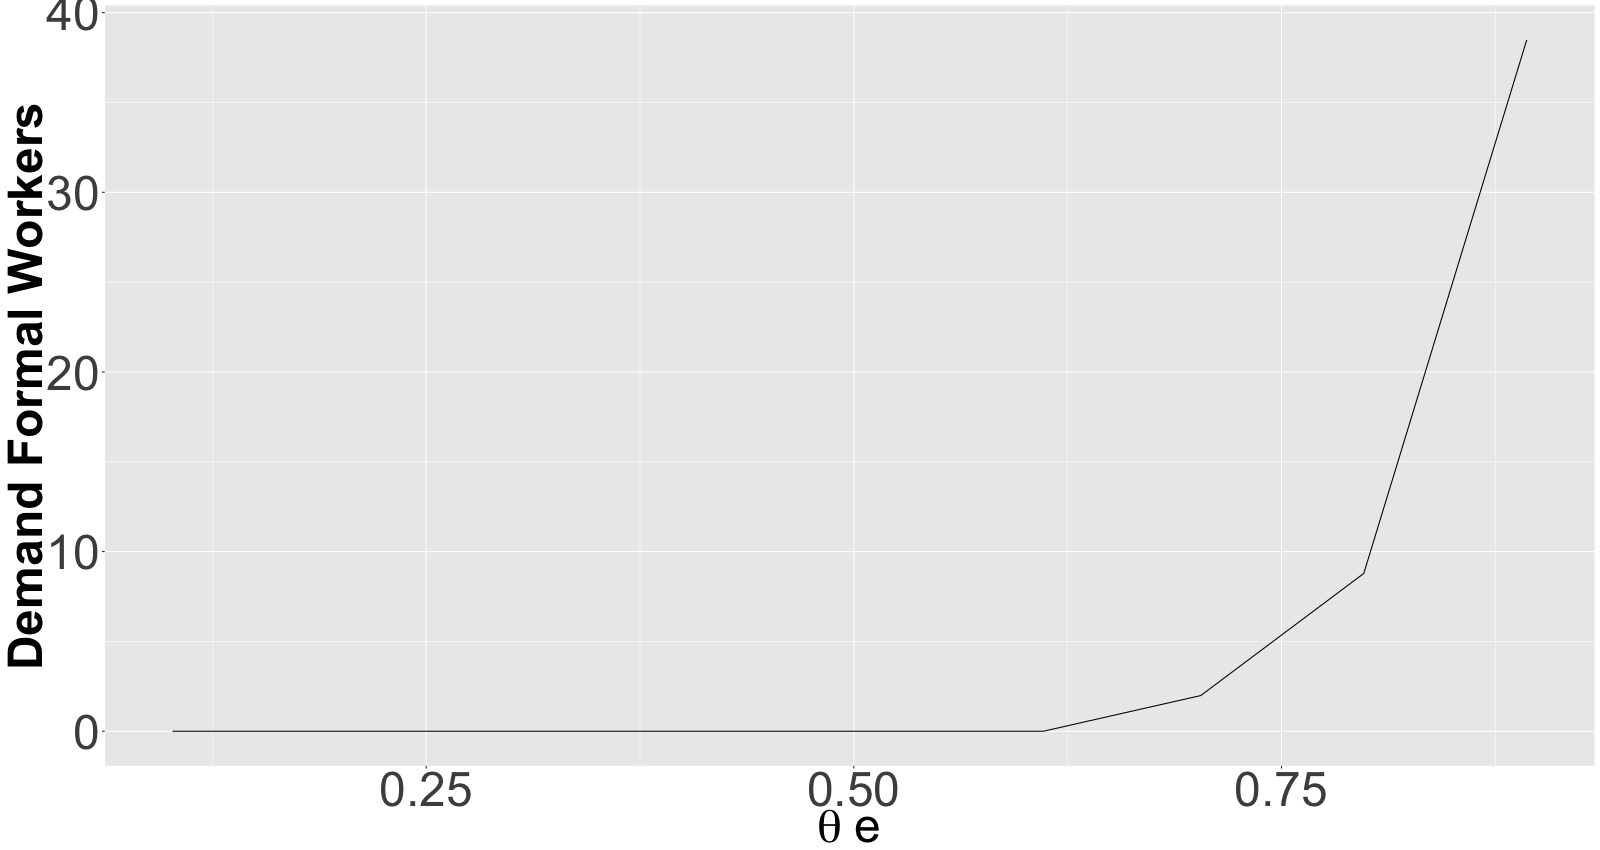
\includegraphics[width=1\textwidth]{/Users/rodrigoazuero/Dropbox/OptmalTaxationShared/Data/git/OptimalTaxation/TheoreticalMoments/FormalDemandPercentile.png}

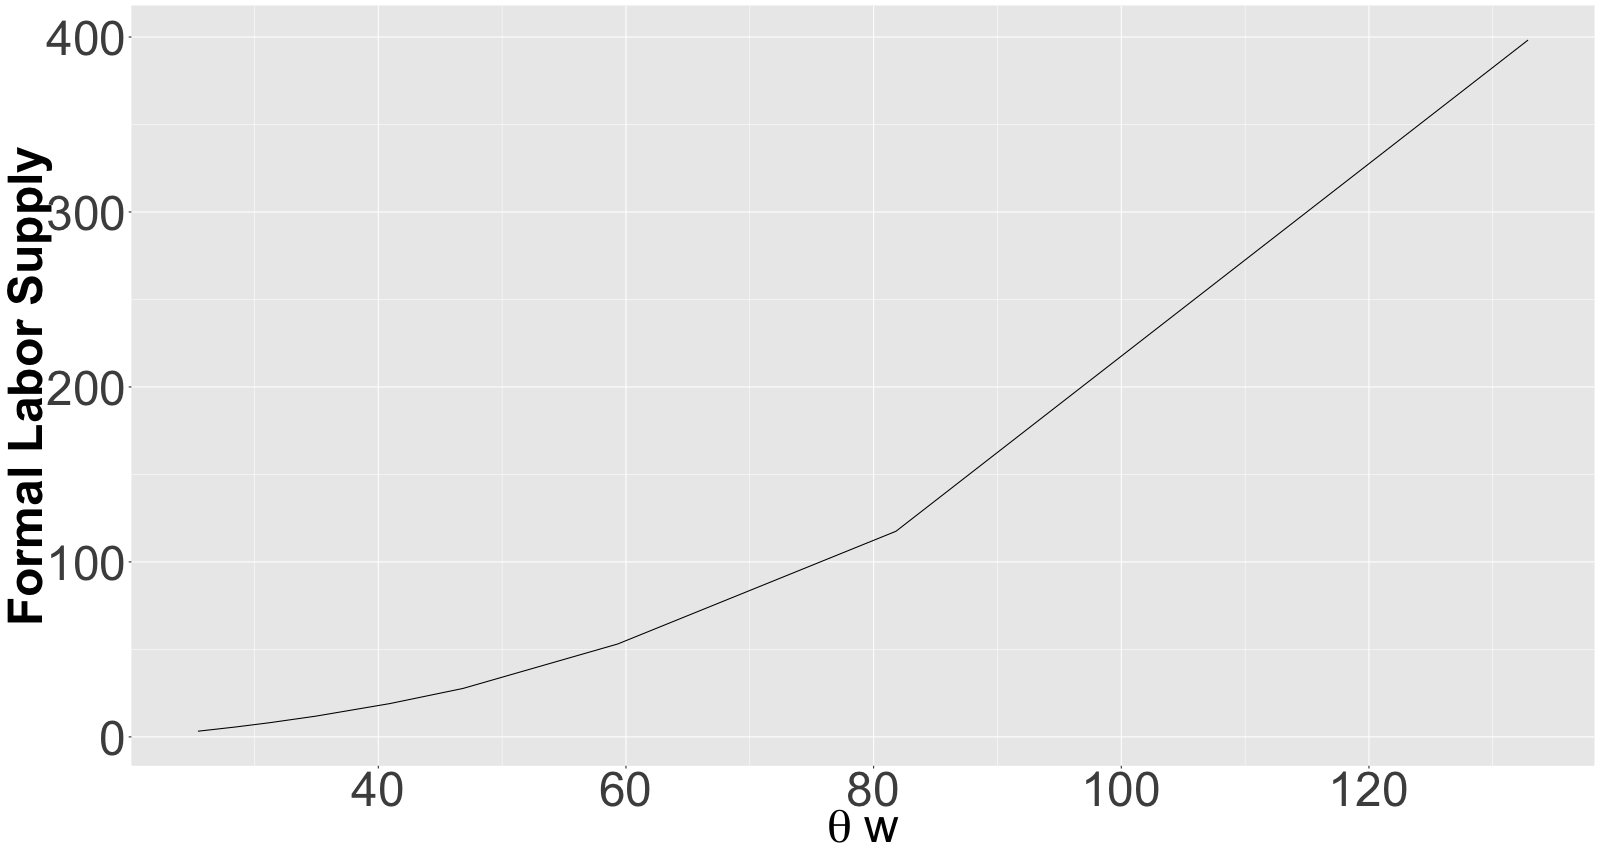
\includegraphics[width=1\textwidth]{/Users/rodrigoazuero/Dropbox/OptmalTaxationShared/Data/git/OptimalTaxation/TheoreticalMoments/FormalSupply.png}

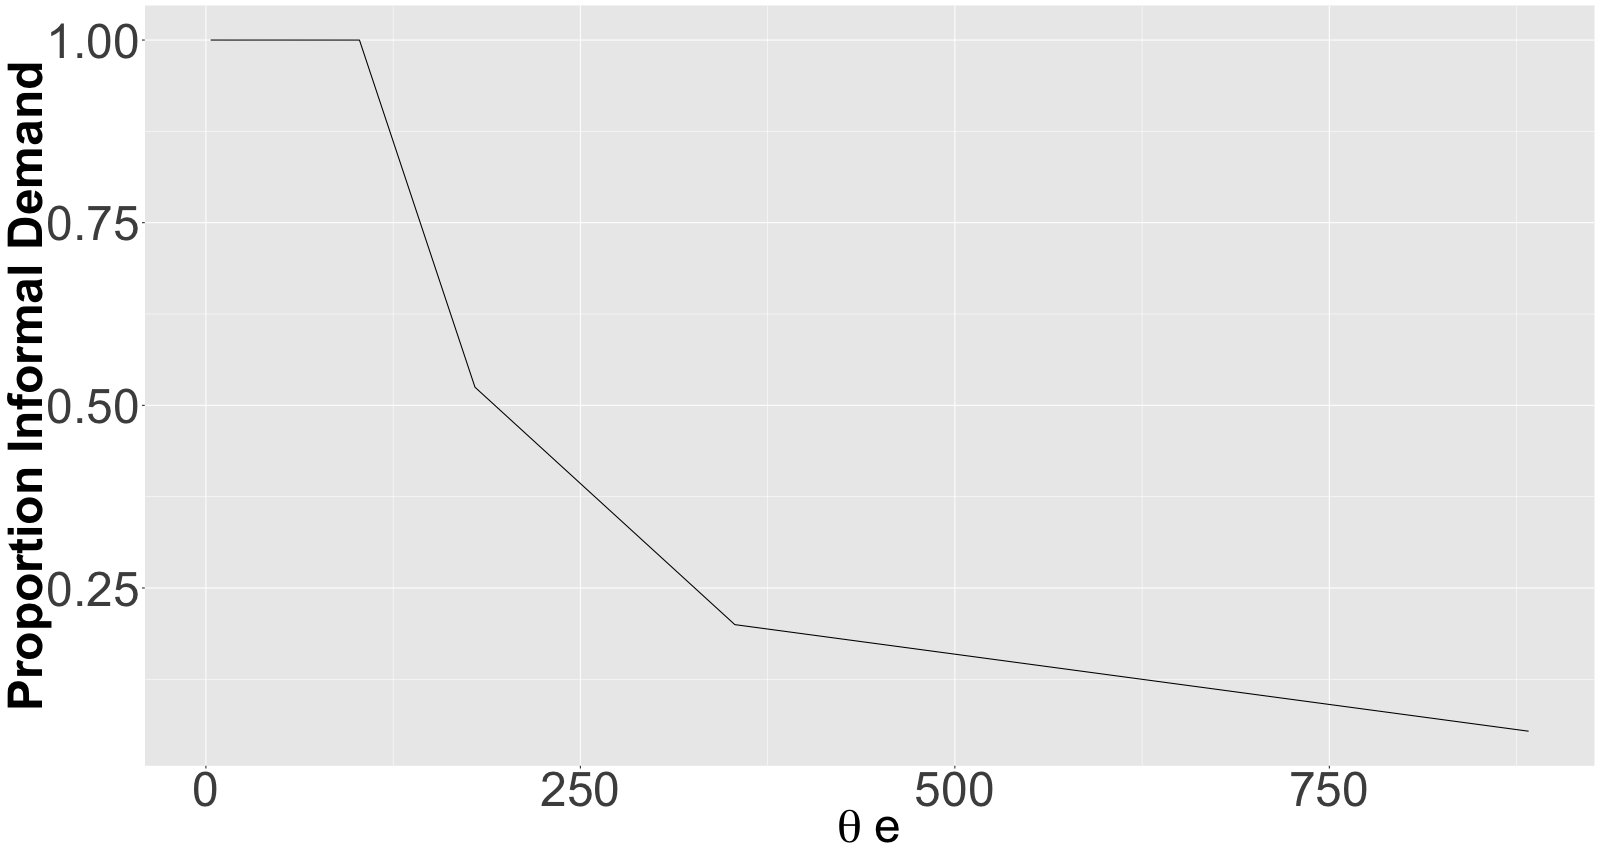
\includegraphics[width=1\textwidth]{/Users/rodrigoazuero/Dropbox/OptmalTaxationShared/Data/git/OptimalTaxation/TheoreticalMoments/InformalProportionDemand.png}


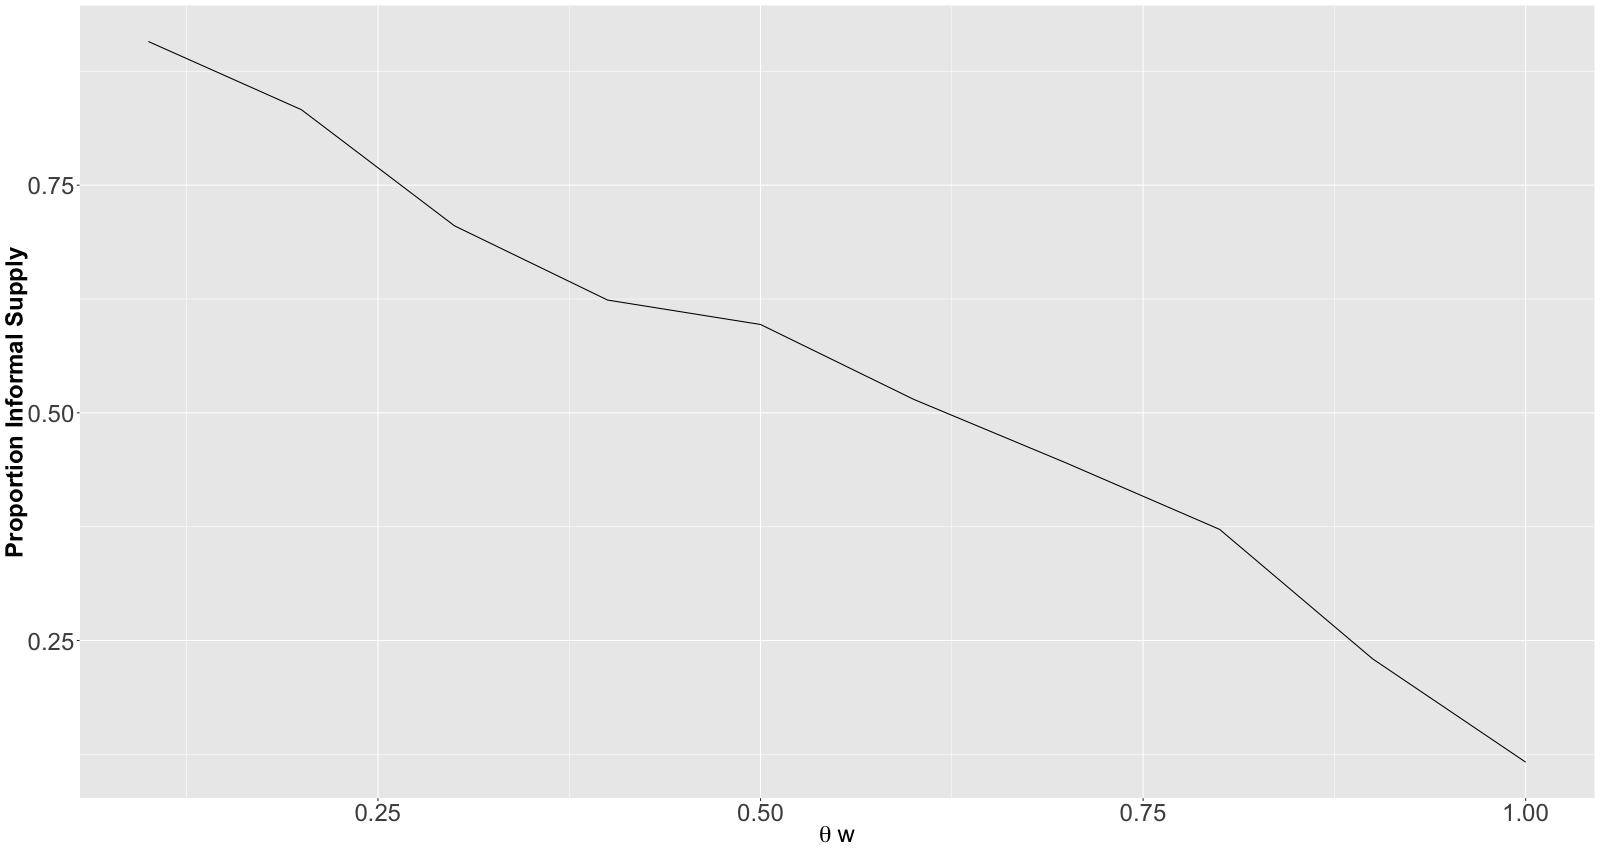
\includegraphics[width=1\textwidth]{/Users/rodrigoazuero/Dropbox/OptmalTaxationShared/Data/git/OptimalTaxation/TheoreticalMoments/InformalProportionSupplyPercentiles.png}
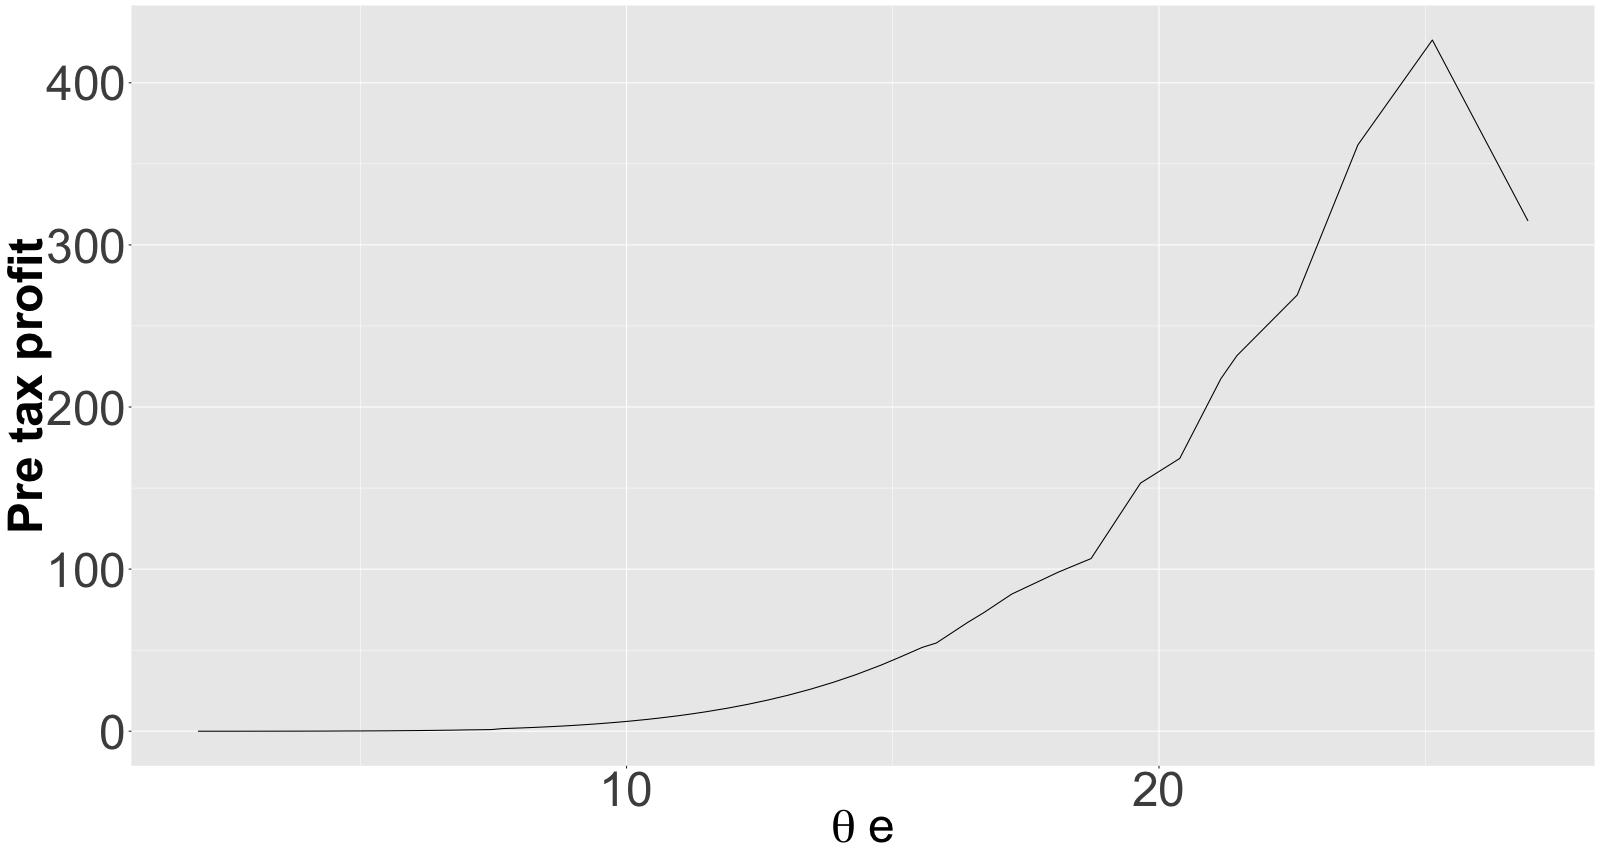
\includegraphics[width=1\textwidth]{/Users/rodrigoazuero/Dropbox/OptmalTaxationShared/Data/git/OptimalTaxation/TheoreticalMoments/PretaxProfit.png}

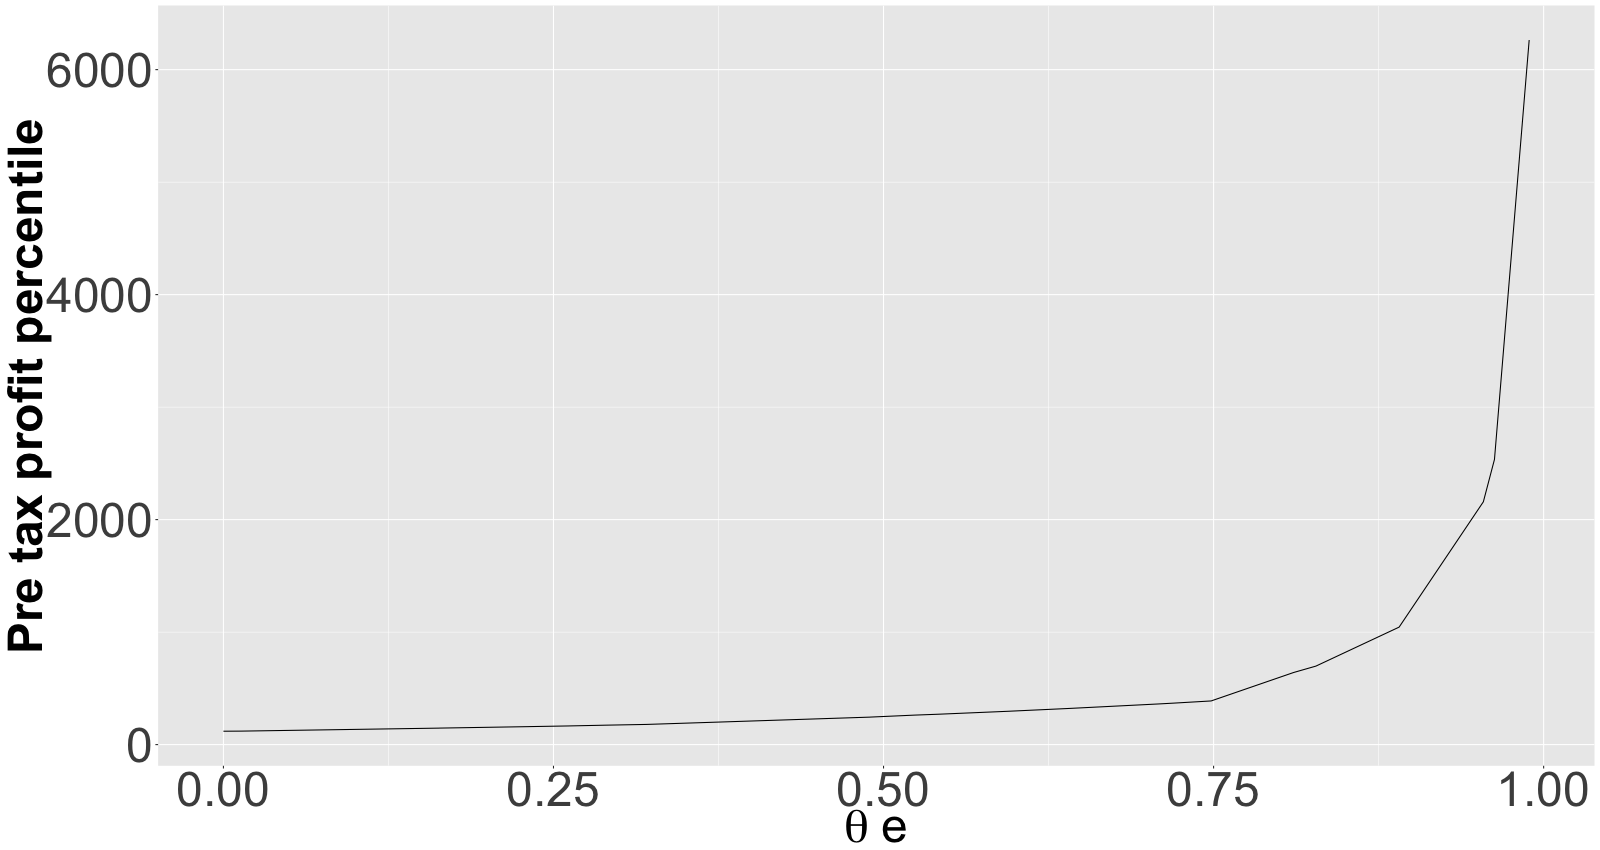
\includegraphics[width=1\textwidth]{/Users/rodrigoazuero/Dropbox/OptmalTaxationShared/Data/git/OptimalTaxation/TheoreticalMoments/PretaxProfitPercentile.png}

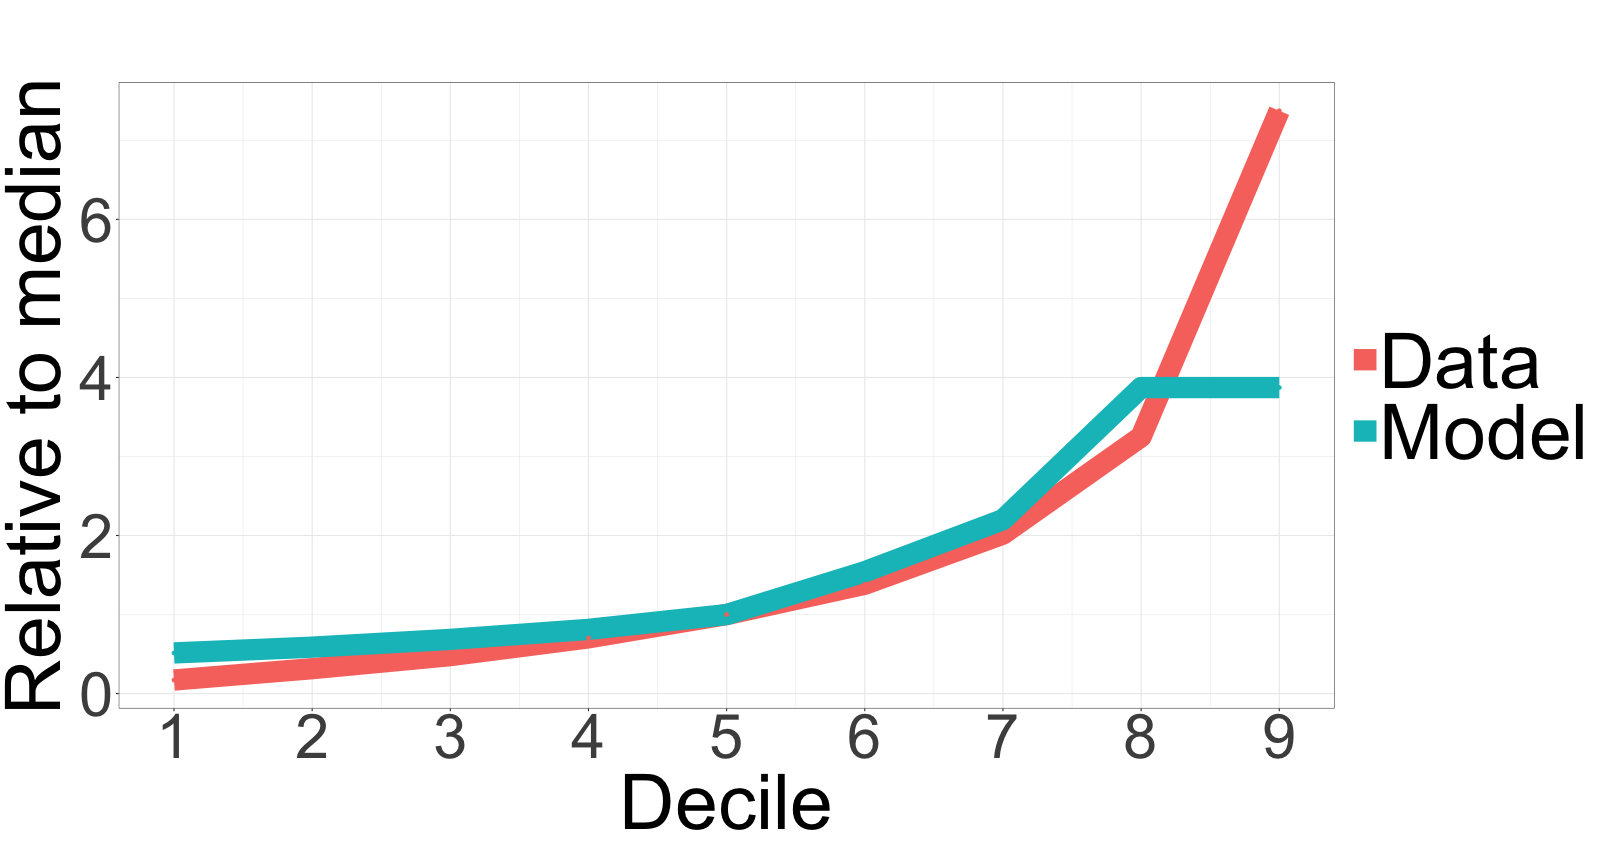
\includegraphics[width=1\textwidth]{/Users/rodrigoazuero/Dropbox/OptmalTaxationShared/Data/git/OptimalTaxation/TheoreticalMoments/Production.png}

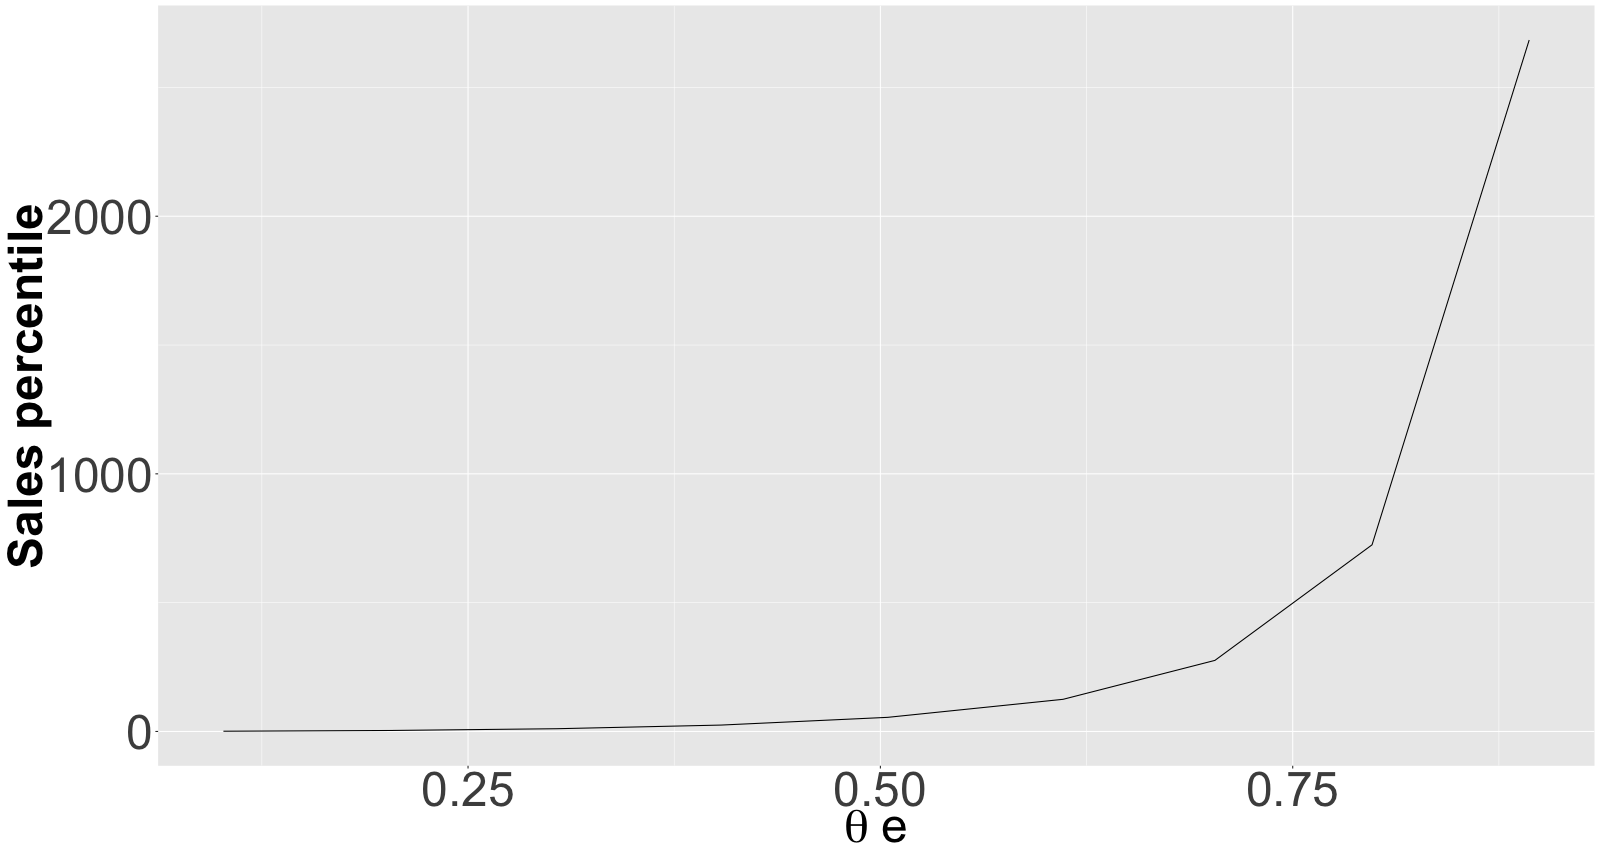
\includegraphics[width=1\textwidth]{/Users/rodrigoazuero/Dropbox/OptmalTaxationShared/Data/git/OptimalTaxation/TheoreticalMoments/ProductionPercentile.png}

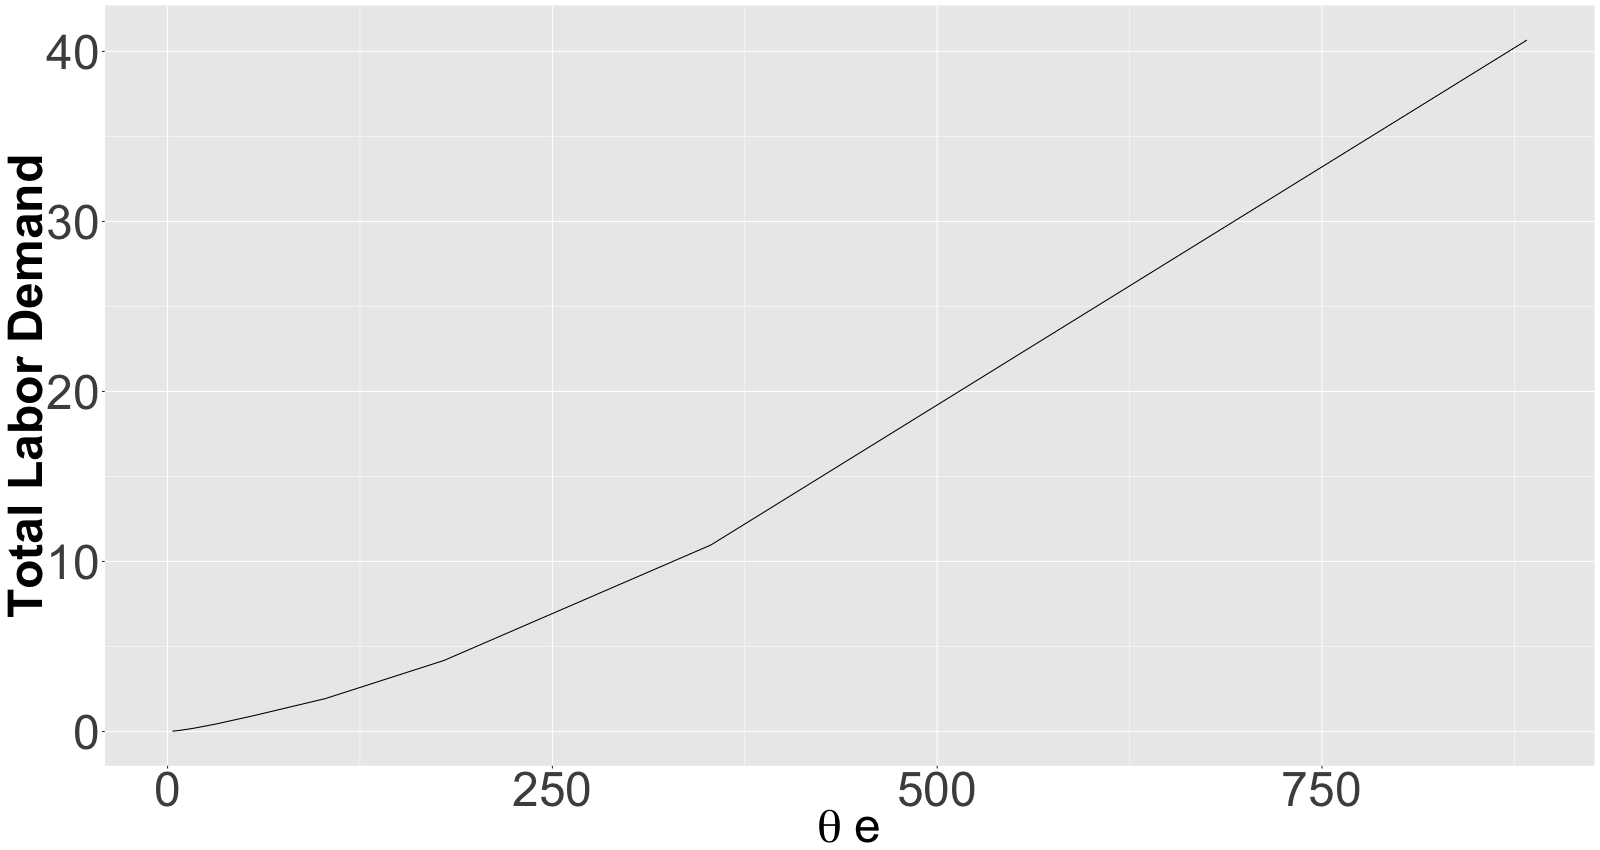
\includegraphics[width=1\textwidth]{/Users/rodrigoazuero/Dropbox/OptmalTaxationShared/Data/git/OptimalTaxation/TheoreticalMoments/TotalLaborDemand.png}

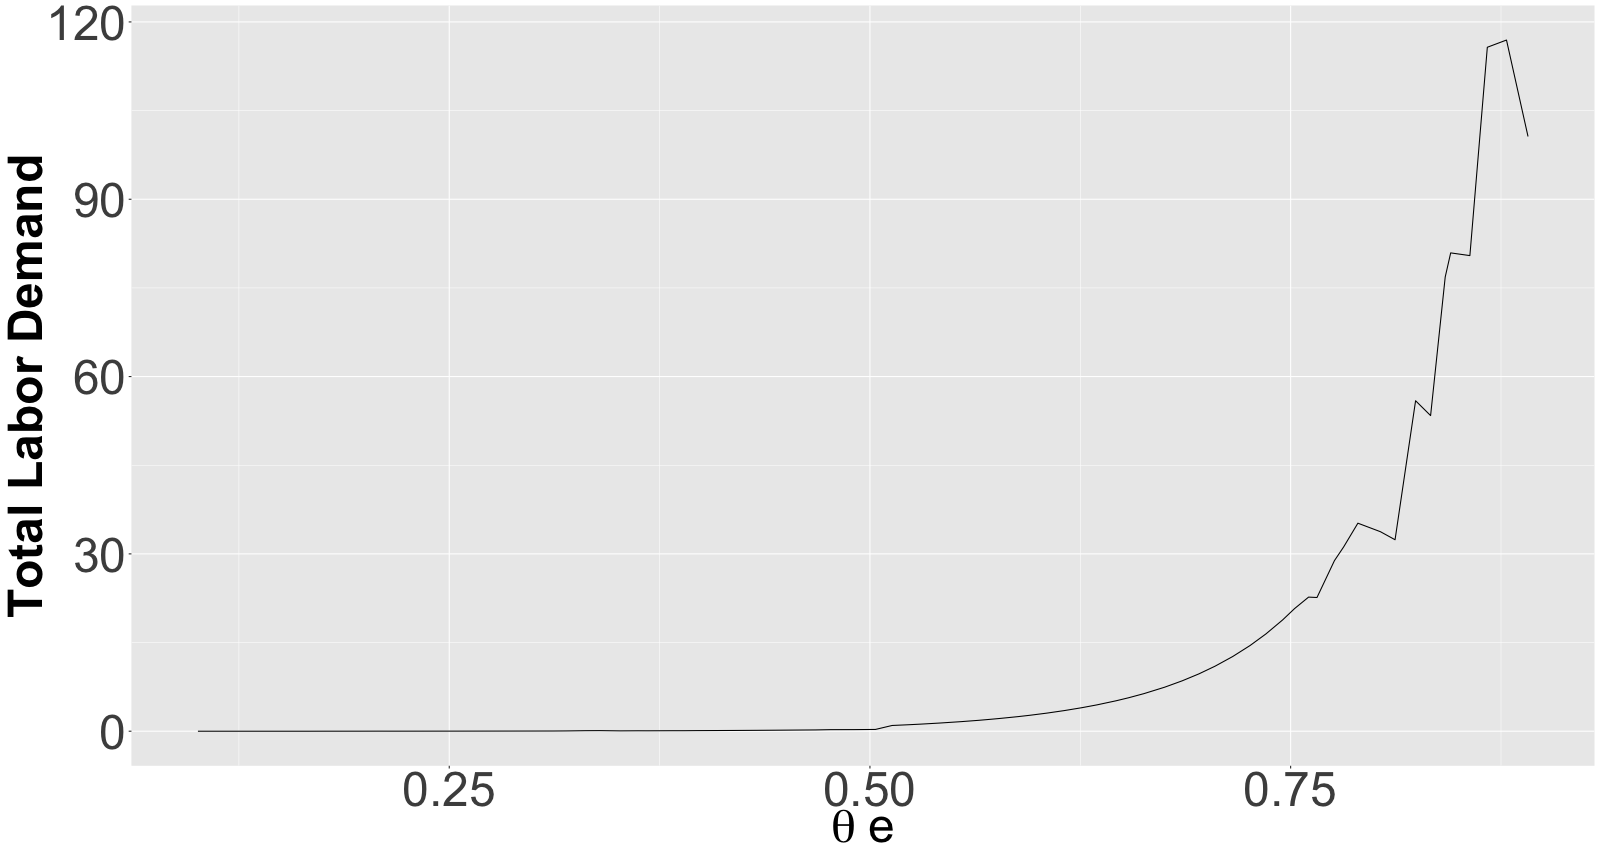
\includegraphics[width=1\textwidth]{/Users/rodrigoazuero/Dropbox/OptmalTaxationShared/Data/git/OptimalTaxation/TheoreticalMoments/TotalLaborDemandPercentile.png}

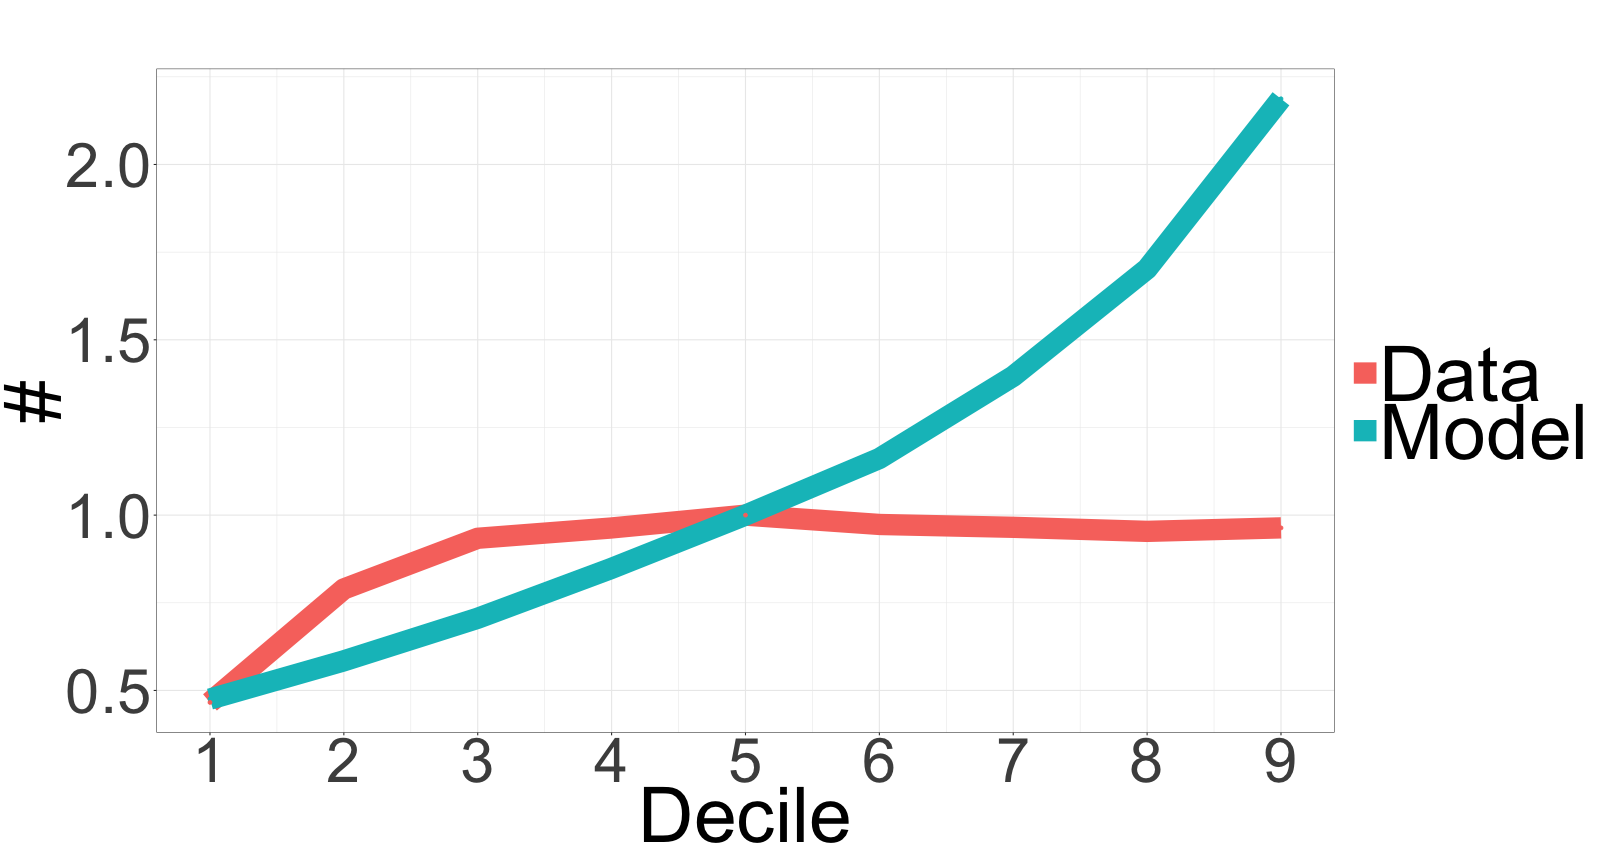
\includegraphics[width=1\textwidth]{/Users/rodrigoazuero/Dropbox/OptmalTaxationShared/Data/git/OptimalTaxation/TheoreticalMoments/TotalLaborSupply.png}


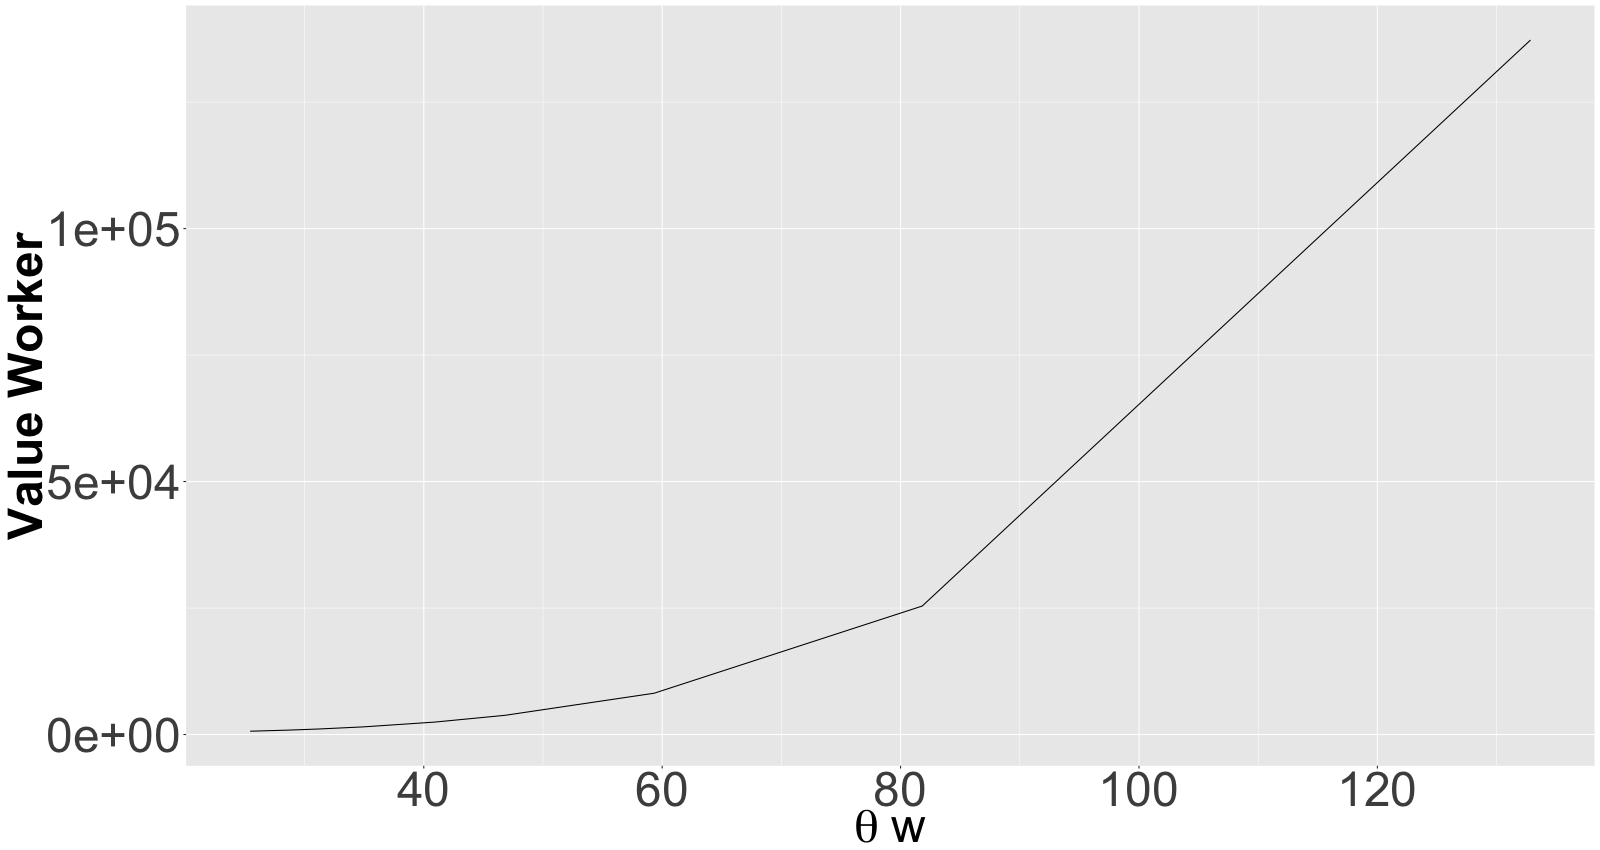
\includegraphics[width=1\textwidth]{/Users/rodrigoazuero/Dropbox/OptmalTaxationShared/Data/git/OptimalTaxation/TheoreticalMoments/ValueWorker.png}

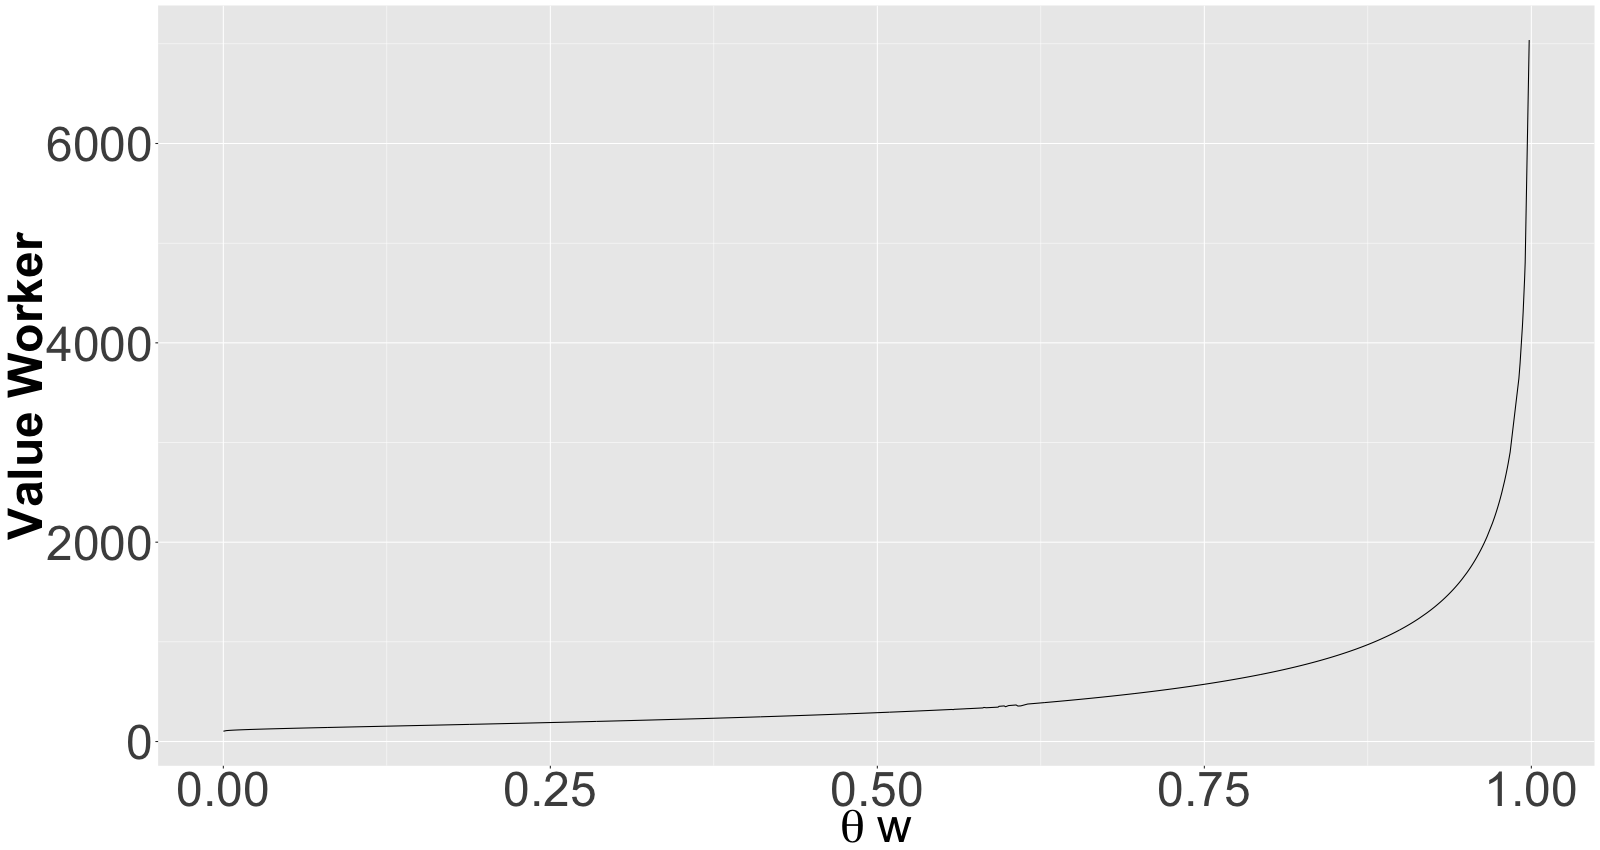
\includegraphics[width=1\textwidth]{/Users/rodrigoazuero/Dropbox/OptmalTaxationShared/Data/git/OptimalTaxation/TheoreticalMoments/ValueWorkerPercentiles.png}

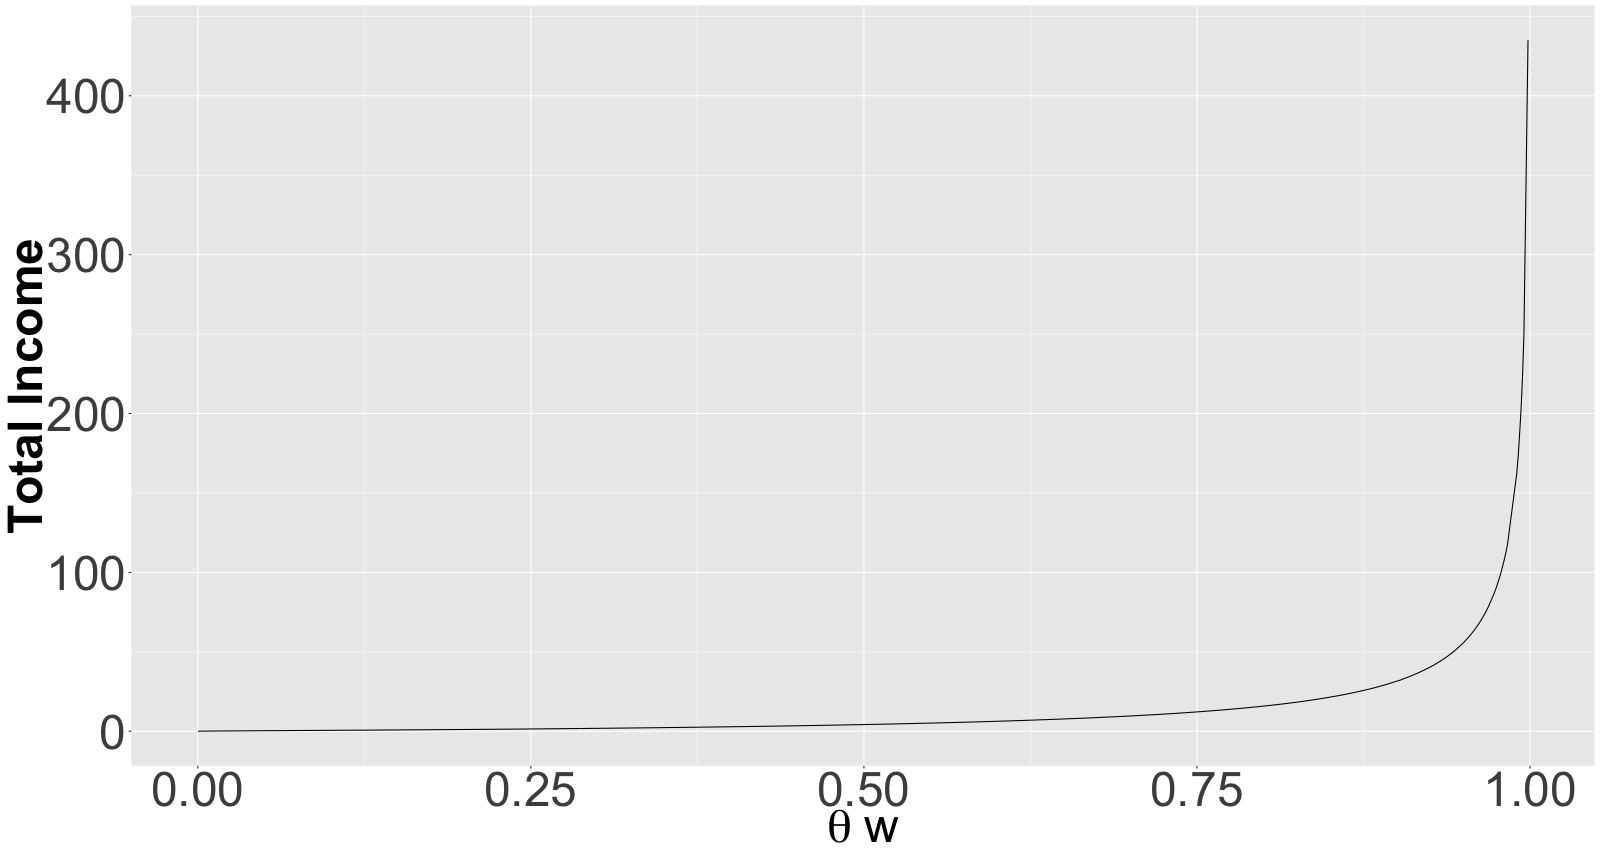
\includegraphics[width=1\textwidth]{/Users/rodrigoazuero/Dropbox/OptmalTaxationShared/Data/git/OptimalTaxation/TheoreticalMoments/TotalIncomePercentiles.png}


\section{Tax functions}
\subsection{CIT}
\begin{align}
\text{CIT}=\
\begin{cases} 0 \text{ if } (p-z)\leq 0
\\  0.756 \text{ if } 0\leq (p-z)\leq 189
\\ 1.89 \text{ if } 189\leq (p-z)\leq 302.1
\\ 7.56 \text{ if } 302.1\leq (p-z)\leq 491.4
\\ 15.12 \text{ if } 491.4\leq (p-z)\leq 756
\\ 22.68 \text{ if } 756\leq (p-z)\leq 1,134	
\\ 0.3\times (\pi-z) \text{ if } (p-z)\geq 1,134	
 \end{cases}
 \\
 \text{where } p=\theta_e(n_i+n_f)^{\alpha}
\end{align}

Caveat: There is another tax bracket for $756\leq (p-z)\leq 1,134$. Chose the one with the lowest tax burden. 

\subsection{PIT}
Government programs to households include a variety of programs (valuation of medical insurance, nutritional programs for kids, pensions for orphans, etc.). Decision was to include all transfers from government to households (from survey) + medical subsidy rather than estimating it from statutory rates. Results:

\begin{table}[H]
\centering
\caption{Distribution of average monthly transfers per capita to households, and SIS membership, by labor income per capita} 
\label{tab:SocPrograms}
\begin{tabular}{ccccc}
  \hline
Decile & Labor Income & Direct Transfers & Households in SIS & Income from profit sharing \\ 
  \hline
1.00 & 63.36 & 56.07 & 0.30 & 0.00 \\ 
  2.00 & 137.84 & 21.99 & 0.23 & 0.88 \\ 
  3.00 & 186.56 & 30.68 & 0.24 & 1.55 \\ 
  4.00 & 238.16 & 24.01 & 0.16 & 2.44 \\ 
  5.00 & 289.53 & 22.32 & 0.18 & 5.94 \\ 
  6.00 & 350.13 & 26.06 & 0.12 & 6.29 \\ 
  7.00 & 438.01 & 26.36 & 0.11 & 13.42 \\ 
  8.00 & 562.08 & 46.81 & 0.07 & 23.22 \\ 
  9.00 & 796.91 & 47.92 & 0.04 & 39.75 \\ 
  10.00 & 2034.87 & 55.72 & 0.02 & 132.84 \\ 
   \hline
\end{tabular}
\end{table}

Real tax rates of PIT are:

\begin{align}
PIT^{\text{real}}
\begin{cases}
	0 \text{ if }x \leq 24,000\\
	15\% \text{ if } 24,150\leq x \leq 117,300\\
	21\% \text{ if } 117,300 \leq x \leq 210,450\\
	30\% \text{ if } 1 x \geq 210,450\\
\end{cases}
\end{align}

Tax function used:
\begin{align}
	PIT^{\text{used}}=
	\begin{cases}
		0.1 x-100 \text{ if }x\leq 1,000 \\
		0 \text{ if} 1,000 \leq x \leq 24,000\\
		\frac{x^2}{100,000}-\frac{9}{25} x \text{ if }24,000\leq x\leq 210,450 \\
		0.3 if x\geq 210,450
	\end{cases}
\end{align}

\subsection{Payroll tax}
Used only 0.9\% payed for health insurance. Assumption of complete wedge (9\% of payroll taxes). 
Caveat: worker does not value health insurance, ignores holidays, family subsidy, bonus, etc.


\section{Parameters used at the moment}

\begin{align}
	\alpha=0.8 \\
  \gamma=0.28\\
  \delta=0.12\\
  \beta=0.15\\
  \sigma=0.2\\
  \kappa=0.1\\
  \psi=0.4\\
  \chi=1.5\\
  \rho=0.9\\
  \mu{w}=1.1\\
  \mu{e}=2\\
  \sigma{w}=0.5\\
  \sigma{e}=1.1\\
  \rho_{e,w}=0.3\\
\end{align}



\end{document}


